\def\mytitle{PYTHON PROGRAMMING ON MATRICES}
\def\myauthor{K.Pavan Kumar}
\def\contact{r170850@rguktrkv.ac.in}
\def\mymodule{Future Wireless Communication (FWC)}
\documentclass[10pt, a4paper]{article}
\usepackage[a4paper,outer=1.5cm,inner=1.5cm,top=1.75cm,bottom=1.5cm]{geometry}
\twocolumn
\usepackage{graphicx}
\graphicspath{{./images/}}
\usepackage[colorlinks,linkcolor={black},citecolor={blue!80!black},urlcolor={blue!80!black}]{hyperref}
\usepackage[parfill]{parskip}
\usepackage{lmodern}
\usepackage{tikz}
	\usepackage{physics}
\usepackage{tabularx}
\usepackage{enumitem}
\usetikzlibrary{calc}
\usepackage{gensymb}
\usepackage{amsmath}
\usepackage{amssymb}
\renewcommand*\familydefault{\sfdefault}
\usepackage{watermark}
\usepackage{lipsum}
\usepackage{xcolor}
\usepackage{listings}
\usepackage{float}
\usepackage{titlesec}
\providecommand{\mtx}[1]{\mathbf{#1}}
\titlespacing{\subsection}{1pt}{\parskip}{3pt}
\titlespacing{\subsubsection}{0pt}{\parskip}{-\parskip}
\titlespacing{\paragraph}{0pt}{\parskip}{\parskip}


\newcommand{\myvec}[1]{\ensuremath{\begin{pmatrix}#1\end{pmatrix}}}
\let\vec\mathbf
\lstset{
frame=single, 
breaklines=true,
columns=fullflexible
}
\thiswatermark{\centering \put(0,-110.0){
\includegraphics[scale=0.3]{logo.png}} }
\title{\mytitle}
\author{\myauthor\hspace{1em}\\\contact\\FWC22011\hspace{6.5em}IITH\hspace{0.5em}\mymodule\hspace{6em}Matrix:Circle}
\date{}
\begin{document}
	\maketitle
	\tableofcontents
   \section{Problem}
If one of the diameters of the circle, given by the equation,
$x^2 + y^2-4x+6y-12=0$., is a chord of a circle S, whose centre is at (-3, 2),Then find the radius of S.

\section{Construction}
  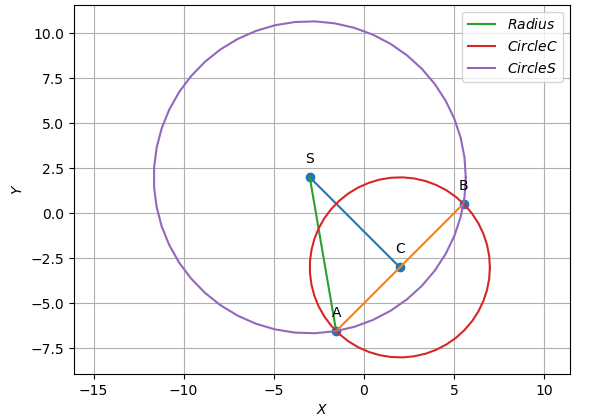
\includegraphics[scale=0.45]{circle.png}
  	\begin{center}
  Figure of construction
  	\end{center}
  \section{Solution}
  Given circle equation : $x^2+y^2-4x+6y-12=0$\\
The standard equation of the conics is given as :
\begin{align}
\vec{x}^{\top}\vec{x}+2\vec{u}^{\top}\vec{x}+f=0
\label{eq:conic}
\end{align}


The given circle  can be expressed in  conics as\\ 
\begin{align}
\vec{u} = \myvec{-2 \\3} , f = -12 
\end{align}
Radius and Centre are
	\begin{align}
	r &=\sqrt{{\vec{u}^{\top}\vec{u}}-f }  ,   \vec{C}=-u
  \end{align}


  
    The steps for constructing above figure are :
\begin{enumerate}
 \item Generate a circle of radius $r$ with centre $\vec{C}$ .
 \item Locate center of another circle  as $\vec{S}$,Join $\vec{C}$ and $\vec{S}$.
 \item Find the Directional vector which is orthogonal to $\vec{S-C}$ say $\vec{m}$.
 \item Find the points of intersection of a line $\vec{x}=\vec{q}+\mu\vec{m}$ with conic passing through $\vec{C}$ ,say $\vec{A}$ and $\vec{B}$.
\item Generate a circle of radius $\norm{S-A}$ or $\norm{S-B}$ with centre $\vec{S}$.
\end{enumerate}


    The input parameters for this construction are
\begin{center}
\begin{tabular}{|c|c|c|}
	\hline
	\textbf{Symbol}&\textbf{Value}&\textbf{Description}\\
	\hline
	$\vec{C}$ &\myvec{2\\-3}&center of circle $\vec{C}$\\
	\hline
    $\vec{S}$ &\myvec{-3\\2}&center of circle $\vec{S}$ \\
	\hline
    $r$ & 5 &Radius of circle $\vec{C}$\\
	\hline
\end{tabular}
\end{center}
\textbf{Theorem:}
A line drawn from the centre of a circle to bisect a chord is perpendicular to the chord.\\

\textbf{Baudhayana Theorem}:In a right-angled triangle, the square of the hypotenuse is equal to the sum of the squares of the other two sides.

\begin{align}
  In   \bigtriangleup SCA:  \angle SCA= 90\degree
\end{align}
By baudhayana theorem,
\begin{align}
 \norm{\vec{S}-\vec{A}}^{2}=\norm{\vec{A}-\vec{C}}^{2}+\norm{\vec{S}-\vec{C}}^{2}
\end{align}
 $\norm{\vec{S}-\vec{A}}$ gives the radius of circle $\vec{S}$ .\\
 $\therefore$ Radius of circle $\vec{S}$ =5$\sqrt{3}$






\textbf{termux commands :}
\begin{lstlisting}
bash circle.sh............using shell command
\end{lstlisting}
\begin{center}
Below python code realizes the above construction :
\fbox{\parbox{8.5cm}{\url{https://github.com/FWC_module1/blob/main/matrices/circle/codes/circle.py}}}
\end{center}
\end{document}
